% ============================================================
% LYCANS TEAM — TRAINEE ASSIGNMENT TEMPLATE
% ============================================================
%

%
% IMPORTANT:
%   This file is intentionally kept simple.
%   Learn the commands and use this template for your work.
%
% ============================================================

% !TeX program = lualatex

\documentclass[11pt,a4paper]{article}

% ------------------------------------------------------------
% BASIC PACKAGES
% ------------------------------------------------------------



\usepackage[a4paper,margin=1in]{geometry}

\usepackage{graphicx}
\usepackage{amsmath}
\usepackage{amssymb}
\usepackage{booktabs}
\usepackage{array}
\usepackage{float}
\usepackage{enumitem}
\usepackage{xcolor}
\usepackage{hyperref}
\usepackage{listings}
\usepackage{siunitx}
\usepackage{caption}
\usepackage{fancyhdr}
\usepackage{lastpage}

% ------------------------------------------------------------
% COLORS
% ------------------------------------------------------------

\definecolor{LycansBlue}{HTML}{002060}
\definecolor{LycansLightBlue}{HTML}{203764}
\definecolor{LycansRed}{HTML}{A20000}
\definecolor{LinkBlue}{HTML}{0563C1}

% ------------------------------------------------------------
% HYPERLINKS
% ------------------------------------------------------------

\hypersetup{
    colorlinks=true,
    linkcolor=LycansBlue,
    urlcolor=LinkBlue,
    citecolor=LycansBlue
}

% ------------------------------------------------------------
% PAGE STYLE
% ------------------------------------------------------------

\pagestyle{fancy}
\fancyhf{}

% Header
\fancyhead[L]{
    \raisebox{-0.15cm}{%
        
\includegraphics[height=0.8cm]{images/lycans-logo.png}%
    }
}

\fancyhead[R]{
    \textcolor{LycansBlue}{\textbf{Trainee Assignment}}
}

% Footer
\fancyfoot[C]{
    Page \thepage\ of \pageref{LastPage}
}

\renewcommand{\headrulewidth}{0.4pt}

% ------------------------------------------------------------
% SECTION STYLE
% ------------------------------------------------------------

\usepackage{titlesec}

\titleformat{\section}
    {\Large\bfseries\color{LycansBlue}}
    {\thesection}
    {0.6em}
    {}

\titleformat{\subsection}
    {\large\bfseries\color{LycansLightBlue}}
    {\thesubsection}
    {0.5em}
    {}

\titleformat{\subsubsection}
    {\normalsize\bfseries\color{LycansBlue}}
    {\thesubsubsection}
    {0.5em}
    {}

% ------------------------------------------------------------
% CODE STYLE
% ------------------------------------------------------------

\lstset{
    basicstyle=\ttfamily\small,
    breaklines=true,
    frame=single,
    columns=fullflexible
}

% ============================================================
% DOCUMENT
% ============================================================

\begin{document}

% ------------------------------------------------------------
% TITLE
% ------------------------------------------------------------

\begin{center}

    {\Large\bfseries\color{LycansBlue}
    LYCANS AERODESIGN TEAM}

    \vspace{0.5cm}

    {\LARGE\bfseries
    PADA Report}

    \vspace{0.5cm}

    \begin{tabular}{rl}
        \textbf{Group Number:} & 02 \\
    \end{tabular}

\end{center}

\vspace{0.5cm}

\hrule

\vspace{0.5cm}

% The final report shall document the team’s engineering process from conceptual design to the final
% aircraft design and assessment.
% The complete report, including figures, tables, references, and appendices, but excluding the
% cover page and table of contents, shall not exceed 15 pages.

\section{Conceptual Design}
\subsection{Mission Requirements and Design Constraints}
Mission Objective is to design a small unmanned aerial vehicle (UAV) resembling the Powered Autonomous Delivery Aircraft, aka PADA. The aim of the project is to simulate both aircraft design
and manufacturing processes, which will follow when the season begins. Designing the aircraft
means working on the wing, tail, fuselage, and electrical system.

The mission has very clear constraints:
\begin{table}[H]
    \centering
    \caption{PADA UAV Mission and Design Constraints}
    \label{tab:mission_constraints}

    \begin{tabular}{ll}
        \toprule
        \textbf{Parameter} & \textbf{Constraint} \\
        \midrule
        Maximum Wingspan & 25 in \\ 
        Maximum Gross Weight & 19.5 oz (including electrical system) \\ 
        Payload & Empty Pepsi can (external mechanism) \\ 
        Wing Airfoil Options & E423, S1223, GOE 165, or NACA 2412 \\ 
        Battery Energy Limit & $\le \SI{100}{\watt\hour}$ (LiHV prohibited) \\ 
        Takeoff Ground Distance & \SI{8}{\meter} to \SI{12}{\meter} \\ 
        Takeoff Angle of Attack & $< 35^\circ$ to $40^\circ$ \\ 
        Minimum Cruise Speed & \SI{25}{\meter\per\second} \\ 
        Minimum Turn Bank Angle & $> 60^\circ$ \\ 
        Flight Altitude Range & \SI{50}{\meter} to \SI{100}{\meter} \\ 
        \bottomrule
    \end{tabular}
\end{table}

\subsection{Selected Aircraft Configuration}
\subsubsection{Airfoil Selection}
The chosen airfoil for the PADA's wing is the S1223 Airfoil, this is based on a trade study as seen below:
\begin{figure}[H]
    \centering

    \begin{minipage}{0.45\textwidth}
        \centering
        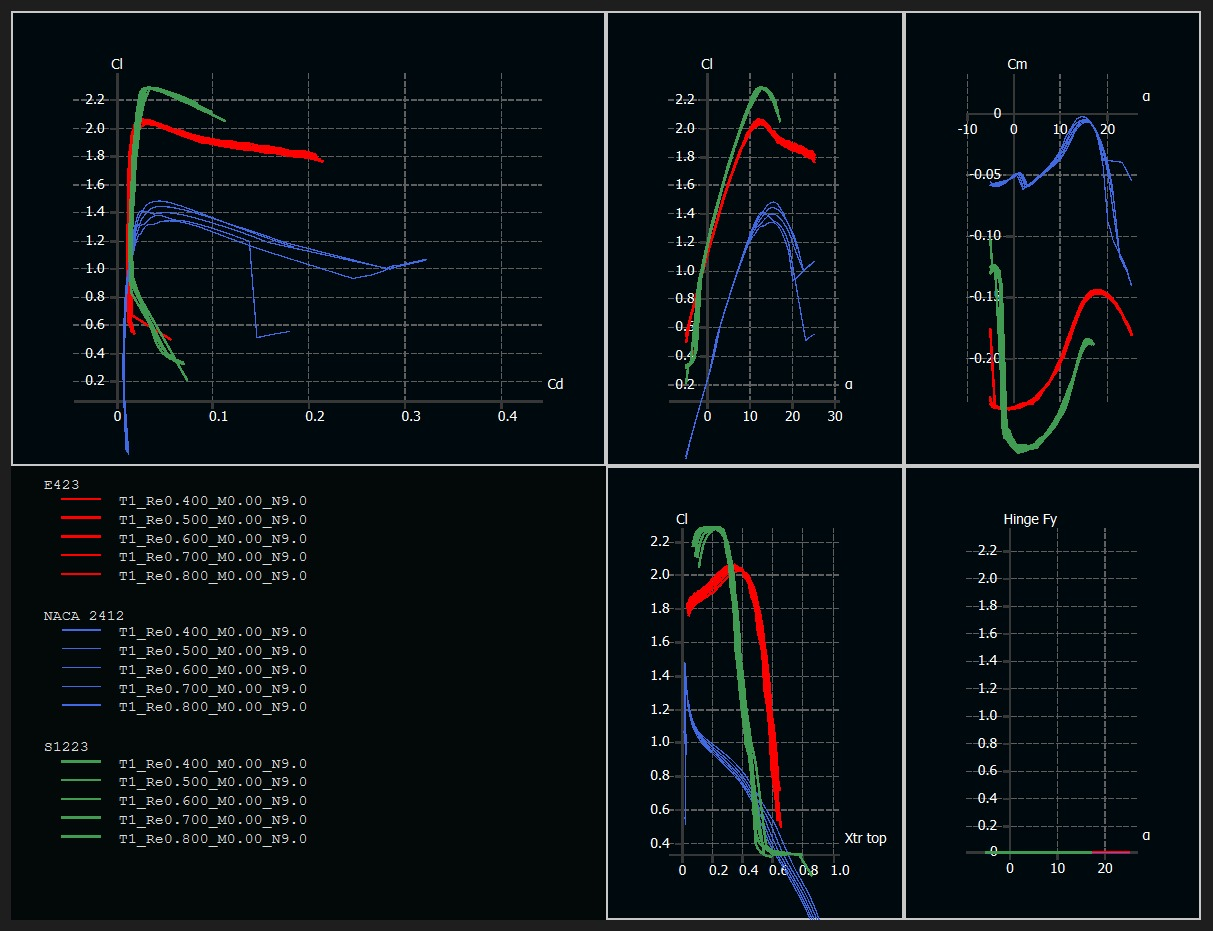
\includegraphics[width=\textwidth]{images/Airfoil Analysis.jpg}
        \caption{Airfoil Analysis and Comparison}
    \end{minipage}
    \hfill
    \begin{minipage}{0.45\textwidth}
        \centering
        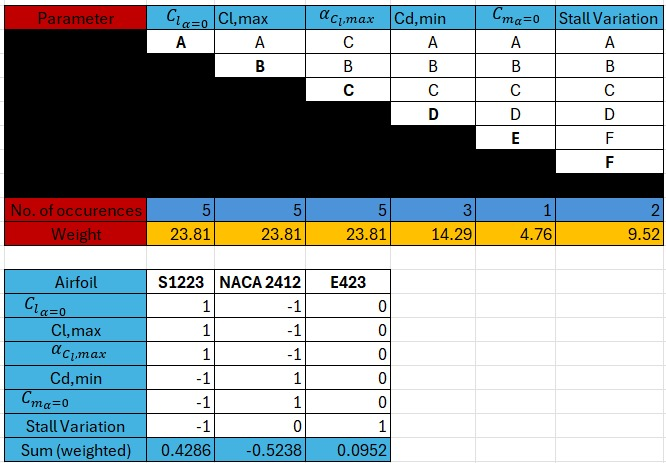
\includegraphics[width=\textwidth]{images/Airfoil Tradestudy.jpg}
        \caption{Airfoil trade study}
    \end{minipage}

\end{figure}

\subsubsection{Wing and Tail Configurations}
\subsubsection{Fuselage}


\section{Preliminary Design}
\subsection{Propulsion Constraint Analysis}
The Constraint Analysis was made based on the Constraints of the mission during Take-off, Cruising, Landing, and Turning, the following is a graph that demonstrates the Analysis:
\begin{figure}[H]
    \centering
    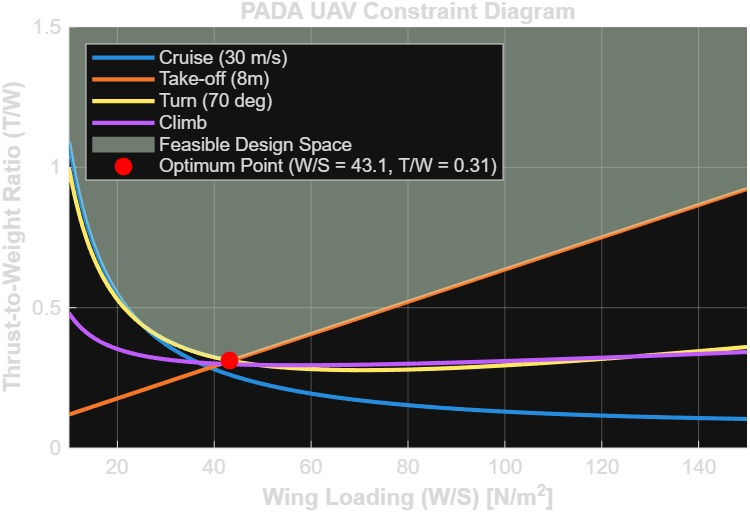
\includegraphics[width=0.6\textwidth]{images/Constraint Analysis.jpg}
    \caption{Propulsion constraint analysis diagram}
    \label{fig:constraint_analysis}
\end{figure}
The optimum point is highlighted where the Wing Loading is 43.1 and the Thrust to weight ratio is 0.31.

This analysis assumes an AR of 3.33 and a Climb rate of 3m/s which will be taken into consideration throughout the project, also R was given a value of 30m to have a smaller turn-radius.
\subsection{Wing and Tail Sizing}

\subsection{Aerodynamic Modeling and Stability Analysis (AVL / XFLR5)}
To evaluate aerodynamic performance and both static and dynamic stability, the sized aircraft was modeled utilizing XFLR5. The initial sizing and geometry were iteratively adjusted to reach a converged, stable design. The mass and center-of-gravity (CG) distribution were also incorporated into the model.

\subsubsection{Design Iterations and Configuration Selection}
A short discussion is required to justify why the final configuration was selected over earlier iterations. Based on manufacturing and aerodynamic constraints, several major modifications were made:
\begin{itemize}
    \item \textbf{Dihedral Angle:} A dihedral angle was initially considered for the main wing. However, it was cancelled in the final design because it proved too difficult to manufacture accurately. The final plane features a flat wing with no dihedral.
    \item \textbf{Tail Arm Length:} Attempts were made to increase the tail arm length to enhance stability margins. This modification increased the horizontal tail volume coefficient ($V_h$) drastically, resulting in overkill stability that would negatively impact pitch authority and maneuverability. Consequently, a normal tail arm length was maintained for the final aircraft.
    \item \textbf{Center of Gravity and Static Margin:} The CG was shifted significantly through multiple iterations to optimize longitudinal stability. Ultimately, the CG was fixed at a location that yields a final static margin of exactly 24\%.
\end{itemize}

\subsubsection{Analysis and Eigenmode Evaluation}
Following the geometric adjustments, dynamic stability analysis was performed to extract the eigenmode values. The output plots and stability modes confirm that the aircraft demonstrates dynamic stability. 


\begin{figure}[H]
    \centering
    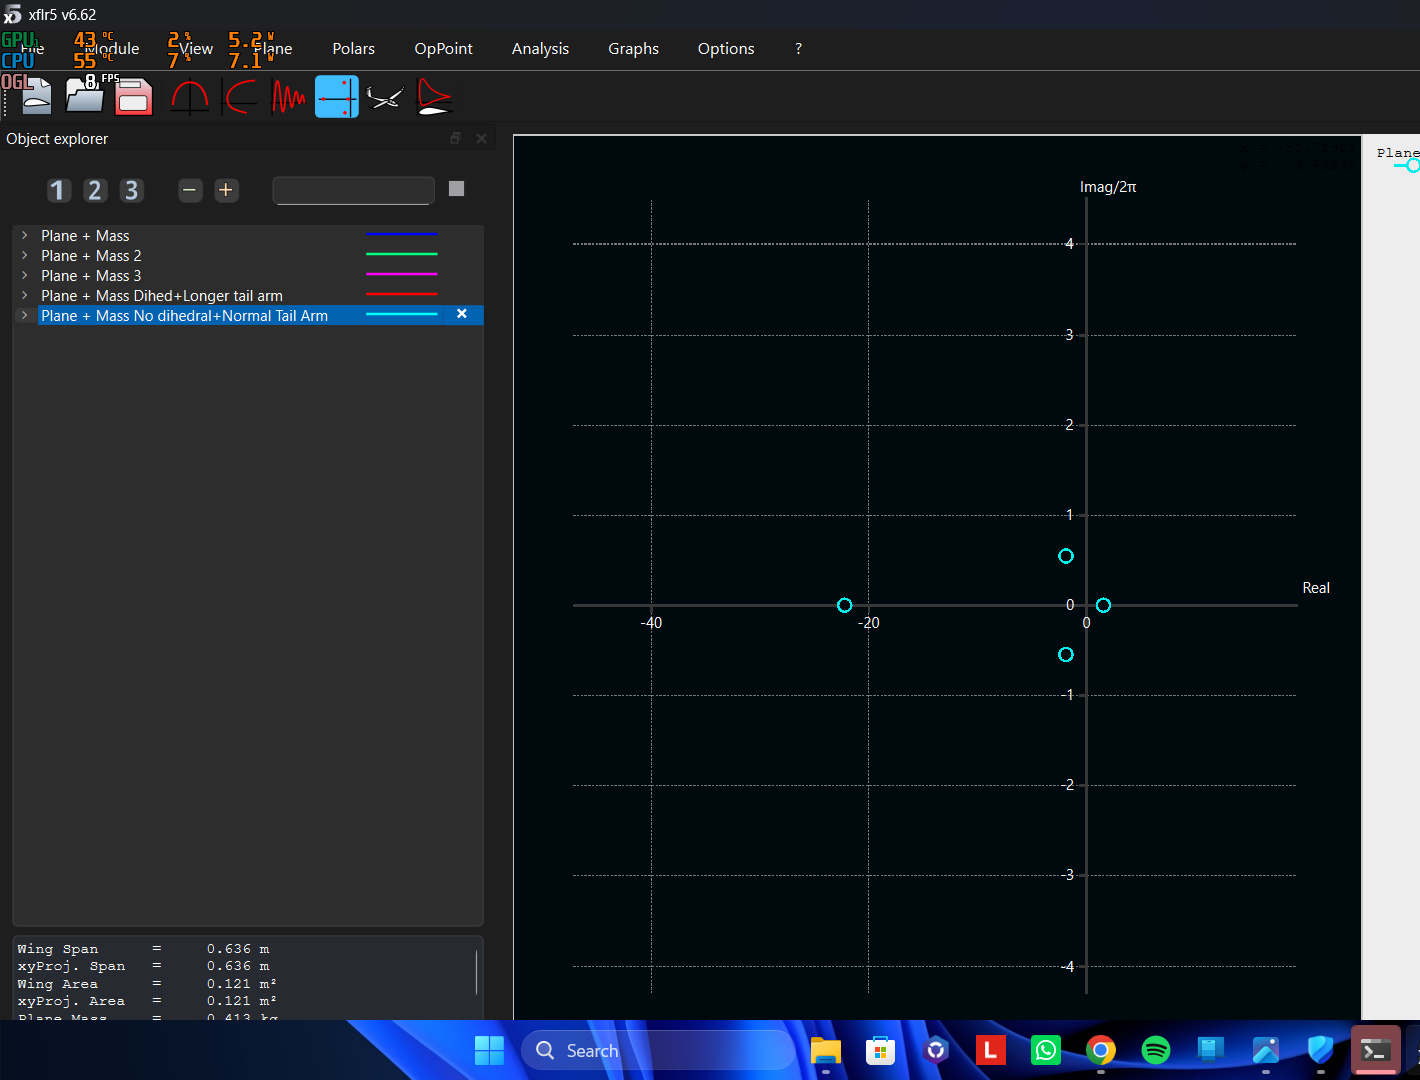
\includegraphics[width=0.6\textwidth]{images/Lateral.png}
    \caption{Dynamic stability eigenmodes and root locus plot from XFLR5. This plot confirms the damping and frequency of short-period modes, verifying the lateral dynamic stability of the final configuration.}
    \label{fig:eigenmodes}
\end{figure}
\begin{figure}[H]
    \centering
    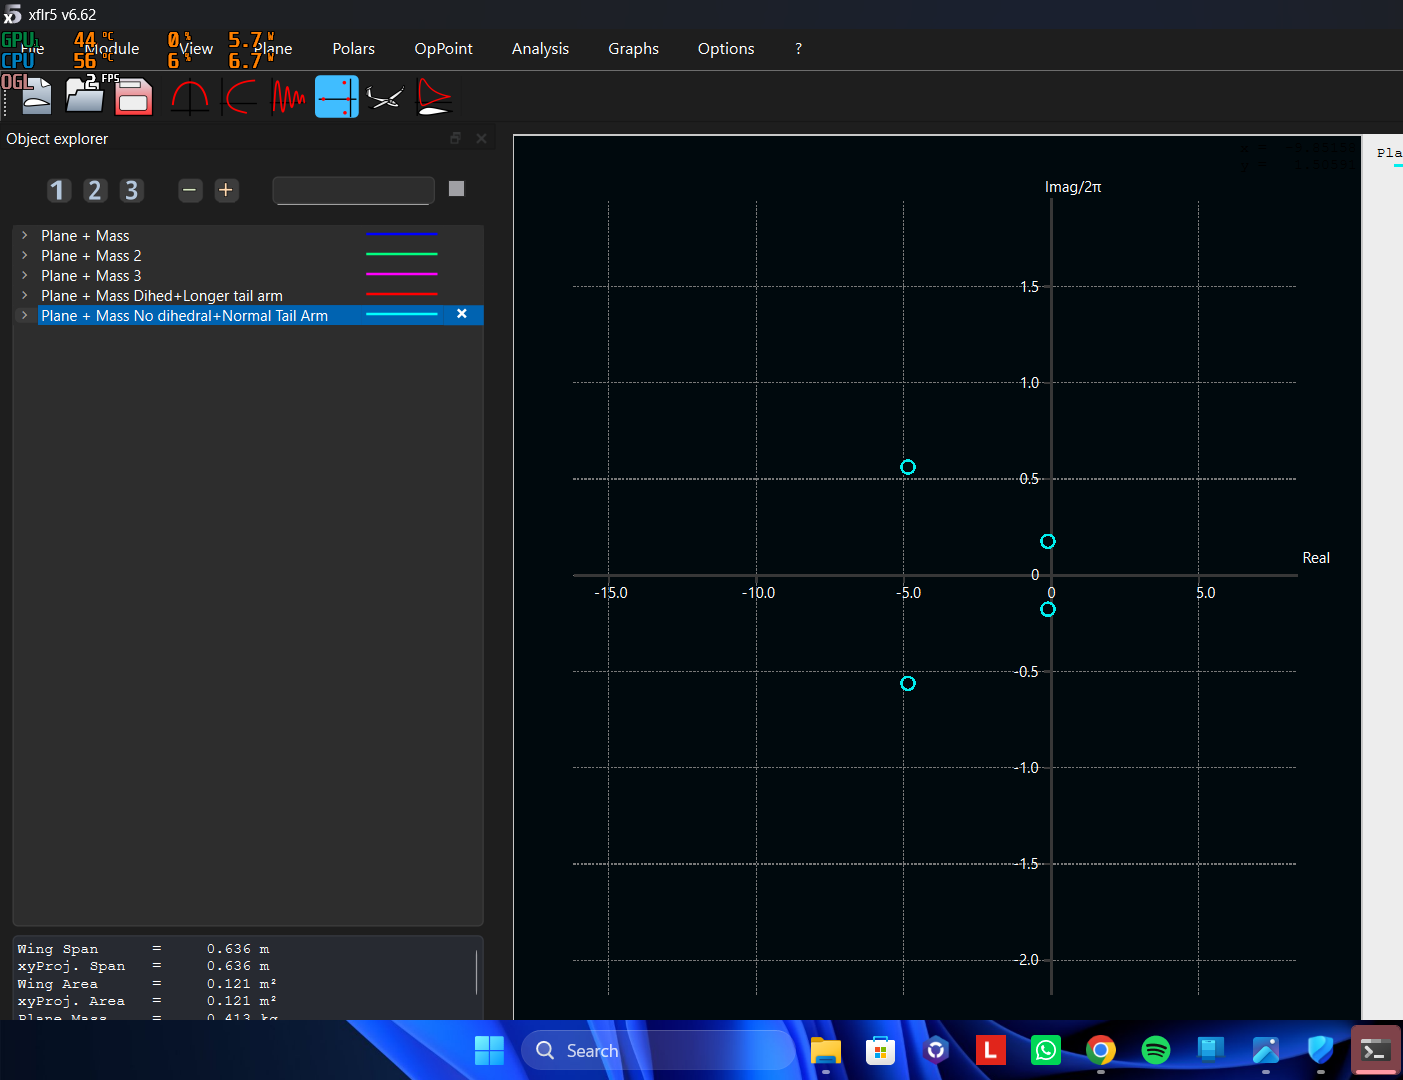
\includegraphics[width=0.6\textwidth]{images/Longitudinal.png}
    \caption{Dynamic stability eigenmodes and root locus plot from XFLR5. This plot confirms the damping and frequency of phugoid modes, verifying the longitudinal dynamic stability of the final configuration.}
    \label{fig:eigenmodes}
\end{figure}
   

\begin{figure}[H]
    \centering
    \includegraphics[width=0.8\textwidth]{images/polars.png}
    \caption{Aerodynamic performance polars. The charts illustrate the lift-to-drag ratios and stability derivatives across varying angles of attack for the final no-dihedral wing configuration.}
    \label{fig:polars}
\end{figure}

\subsection{Aircraft Design}
\begin{figure}[H]
    \centering
     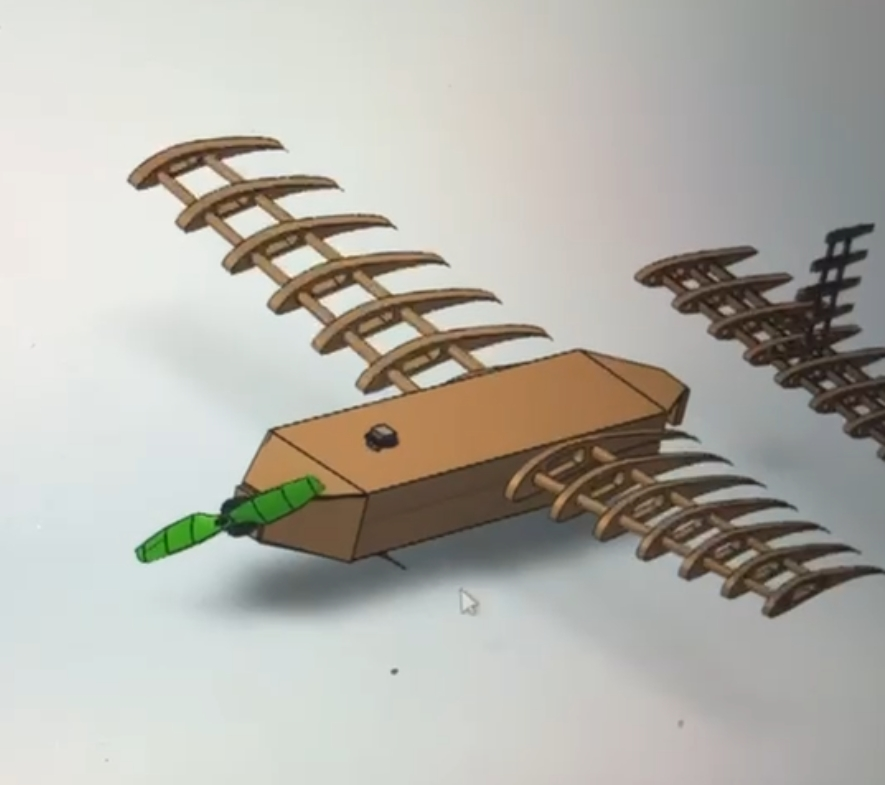
\includegraphics[width=0.8\textwidth]{images/Solid.jpg}
    \caption{Solid works implantation}
    \label{fig:solidworks}
\end{figure}

\begin{figure}[H]
    \centering
     \includegraphics[width=0.8\textwidth]{images/wing.png}
    \caption{Final main wing configuration featuring zero dihedral for optimized manufacturability and structural simplicity.}
    \label{fig:final_wing}
\end{figure}

\begin{figure}[H]
    \centering
    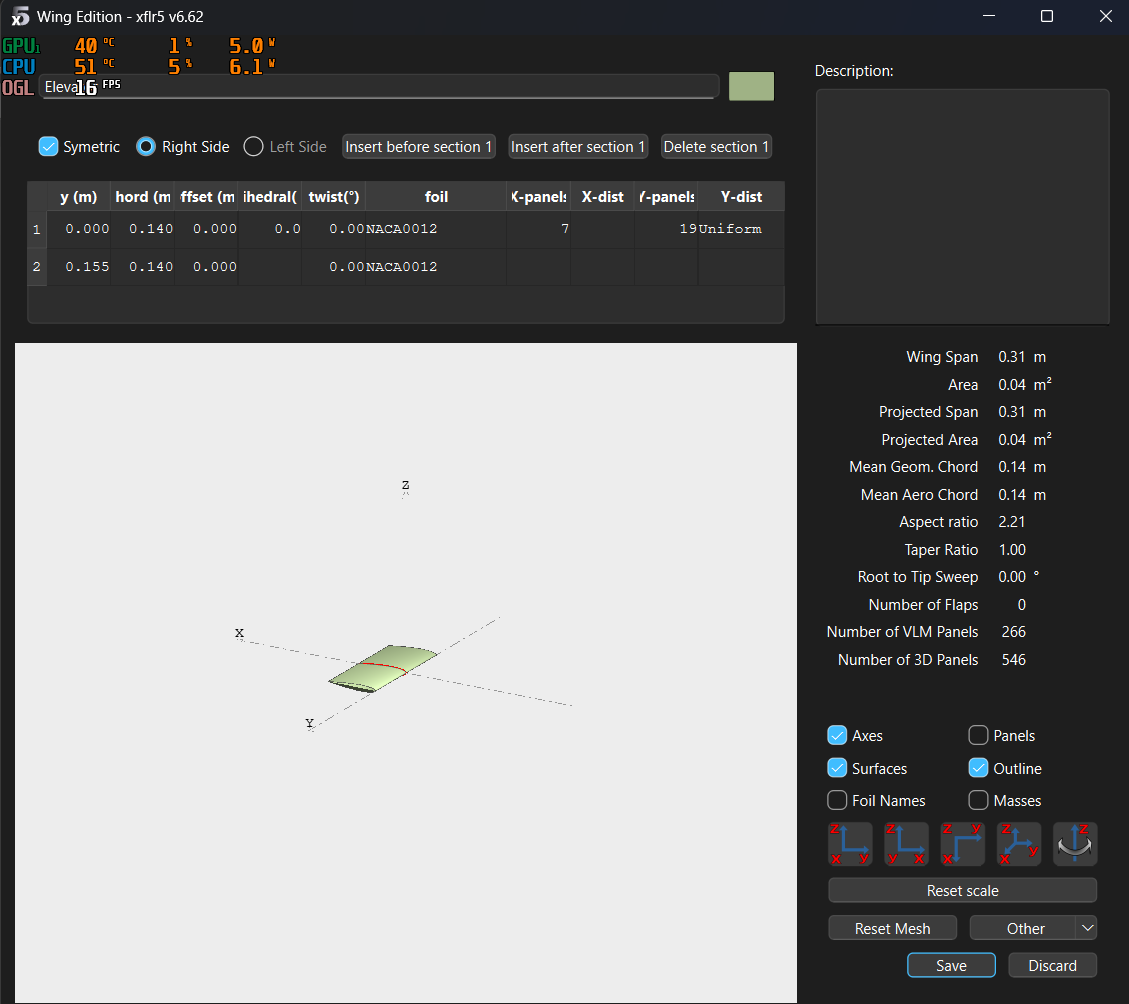
\includegraphics[width=0.4\textwidth]{images/H Tail.png}
    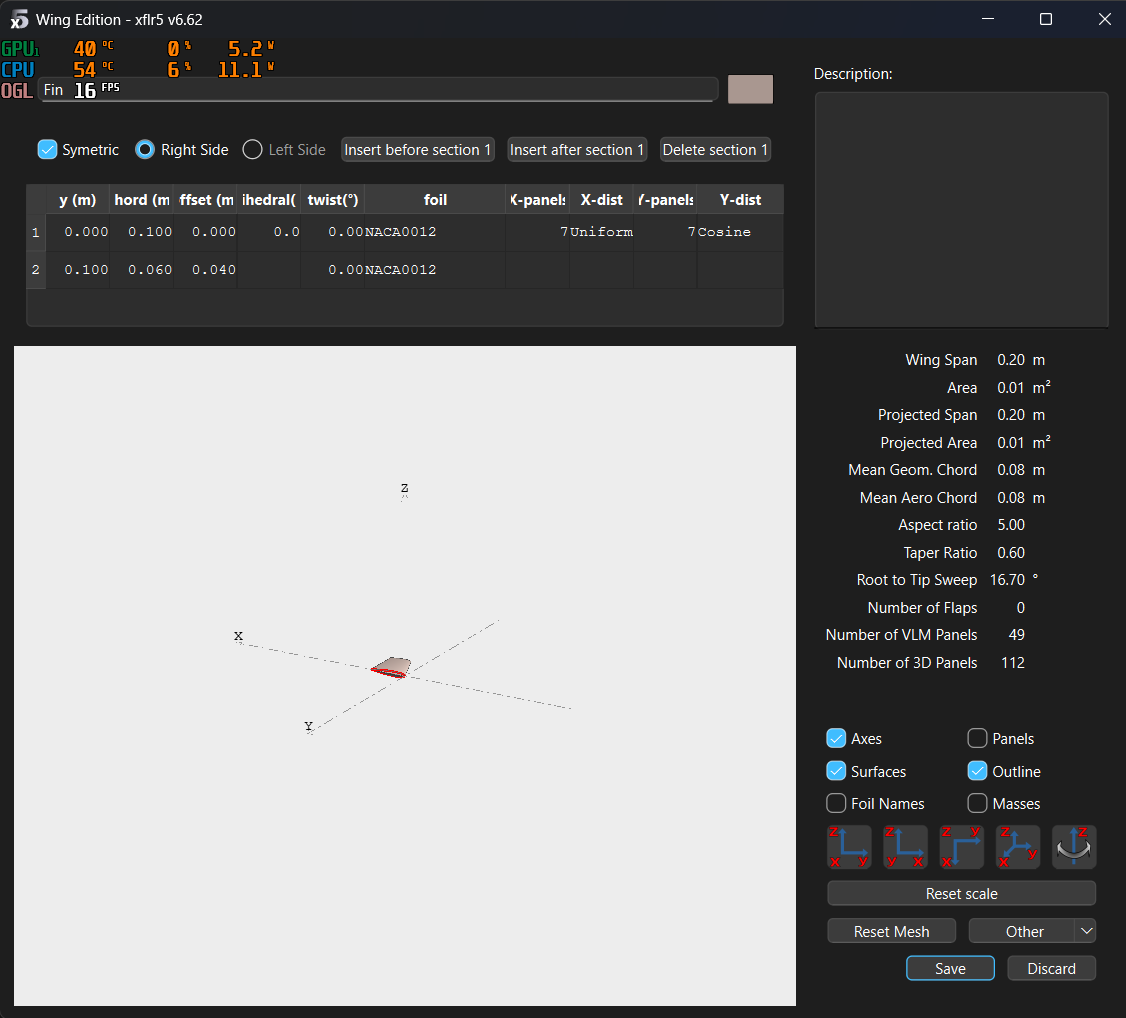
\includegraphics[width=0.4\textwidth]{images/V Tail.png}
    
    \caption{Final empennage design utilizing a normal tail arm length to maintain an optimal horizontal tail volume coefficient ($V_h$) without inducing excessive stability.}
    \label{fig:final_tail}
\end{figure}

\begin{figure}[H]
    \centering
    \includegraphics[width=0.8\textwidth]{images/cg.png}
    \caption{Final Center of Gravity (CG) placement on the aircraft, yielding a 24\% static margin for balanced static stability.}
    \label{fig:final_cg}
\end{figure}

\subsection{Electrical and Avionics Design}
% Include:
% • Electrical system block diagram and schematic.
% • Power budget and component selection.
% • Battery, ESC, motor, propeller, flight controller, GPS, telemetry, servos, and regulators.
% • Wiring, connectors, protection, and electrical safety considerations.
% • Component placement and integration within the aircraft
\subsection{Autonomous System and Software}
% Include:
% • Overall system architecture and data flow.
% • ROS 2 node structure, topics, messages, and MAVROS interfaces, including an rqt_graph
% visualization of the complete ROS 2 communication graph.
% • Visual perception and target-to-flight-mode mapping.
% • Decision-making, obstacle avoidance, and mission recovery.
% • Error handling and relevant performance measurements.
% • Evidence from the SITL demonstration
\subsection{Payload Release Mechanism}

\subsubsection{Final CAD design and release principle.}
\begin{figure}[H]
    \centering
    
\includegraphics[width=0.6\textwidth]{images/Payload Mech.png}
    \caption{All items needed for the payload release mechanism
    }
    \label{fig:payload_mech}
\end{figure}
\begin{itemize}
        \item Movable Arm
        \item Fixed Arm
        \item Back Support
    \end{itemize}
    \textbf{How does it work?} A fifth servo was added to move the controllable arm outwards causing the payload to drop but two arms aren't enough to hold the payload so a third arm was added to the back of the payload to maintain its stability.This mechanism was strategically mounted directly under the final CG to maintain structural balance and ensure the 24\% static margin remains completely unaffected during the payload drop. 
% • Mounting and aircraft integration.
% • Weight, balance, reliability, and manufacturability considerations.


\subsection{Material Selection}
When evaluating candidate materials for the airframe, the primary selection criteria were weight, durability, cost, and availability. Balsa wood was selected as the primary material for all structural components. Balsa provides an excellent strength-to-weight ratio, ensuring the airframe is durable enough to withstand aerodynamic loads while maintaining a low mass to stay well under the maximum gross weight limit. Furthermore, balsa wood is highly cost-effective and was realistically the only viable, accessible material that suited both our manufacturing capabilities and the mission constraints.

\section{Manufacturing Plan}
The manufacturing strategy was designed around rapid prototyping and precise assembly using laser-cut balsa wood. The complete process is outlined as follows:

\begin{itemize}
    \item \textbf{Material Sourcing:} Standard balsa wood planks, specifically dimensioned at $\SI{1000}{\milli\meter} \times \SI{100}{\milli\meter} \times \SI{5}{\milli\meter}$, were procured for the airframe construction.
    \item \textbf{Digital Preparation:} The full 3D CAD assembly was translated into 2D manufacturing instructions. These vector files contained the exact layout for all necessary structural parts, including wing ribs, fuselage formers, and empennage surfaces.

    \begin{figure}[H]
    \centering
    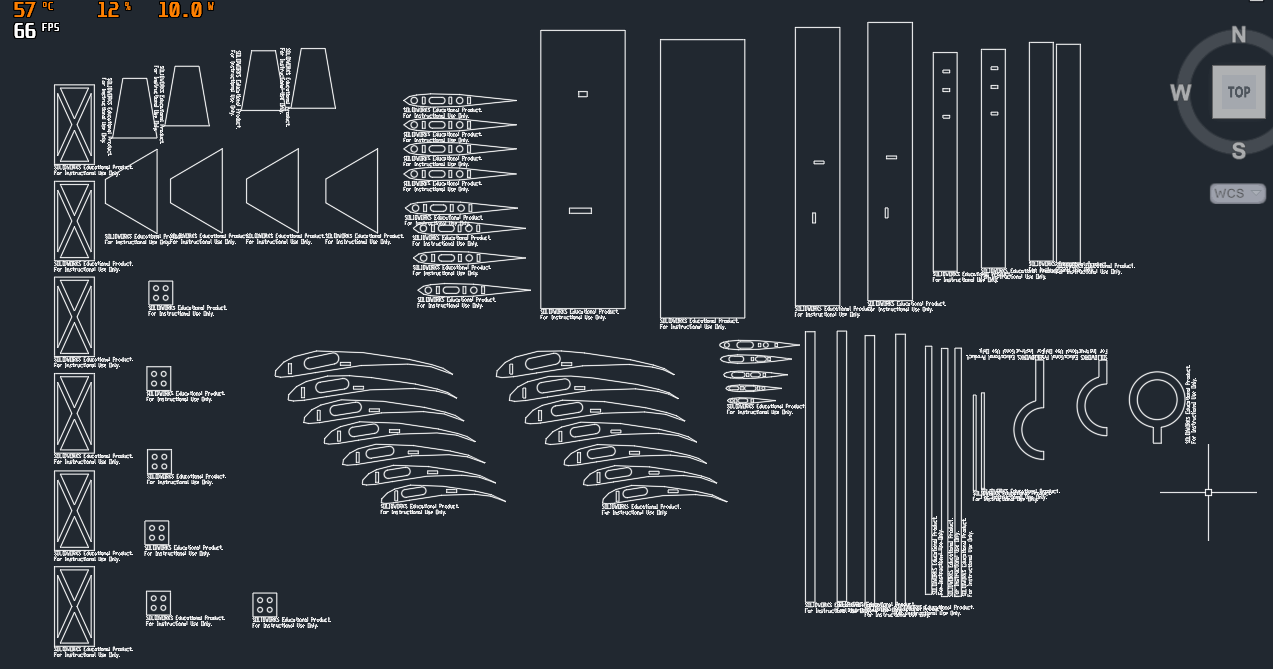
\includegraphics[width=0.6\textwidth]{images/All Components CAD.png}
    \caption{Full 2D manufacturing instructions
    }
    \label{fig:manu inst}
\end{figure}


    \item \textbf{Laser Cutting:} The finalized CAD cutting instructions were sent to the laser cutting facility. Using a laser cutter allowed for extremely high-precision cuts, ensuring that all interlocking tabs and slots would fit together perfectly without requiring excessive manual sanding or modification.
    \item \textbf{Assembly:} After all parts were cut from the balsa planks, they were aligned and glued to form the final airframe structure, preceding the integration of the electrical systems and payload mechanism.
\end{itemize}

\end{document}
